In our first calculation, we take the first trail wave function \ref{eq:t1}.
At beginning, we take $\omega=1.0$ and vary $\alpha$ from 0.675 to 1.15.
The total number MC samplings $N$ is set to be $10^7$.
\begin{figure}[tb]
\label{fig:t1}
\centering
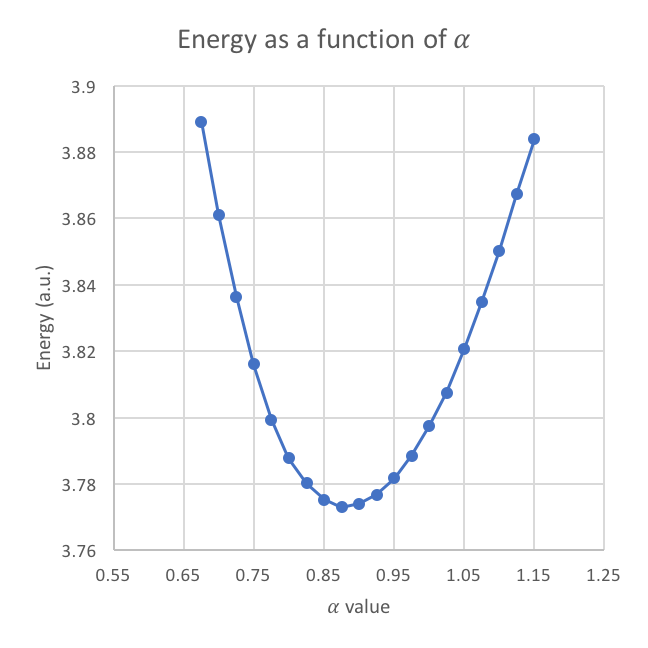
\includegraphics[width=0.4\textwidth]{t1.png}
\caption{Relation between lowest $E$(a.u.) and the variational parameter $\alpha$ where $\omega$ is set to one and $N=10^7$ obtained from $\Phi_{t1}$.}
\end{figure}

In Fig. \ref{fig:t1}, we show lowest energies for different $\alpha$. 
Clearly, it has a minimum value $E_{min}=3.7729\ a.u.$ corresponding to $\alpha=0.875$.
Energies and variances for some $\alpha$ are shown in Table \ref{tab:t1}.
We can see that the accuracy can be improved by sample more points ($N$).
\begin{table}[tb]
	\centering
	\caption{Lowest energies and variances for   different $\alpha$ (partly) where $\omega$ is set to one and $N=10^7$ obtained from $\Phi_{t1}$. All qualities are in atomic unit.}
	\label{tab:t1}
	\begin{tabular}{cccc}
		\hline
		\hline
		$\alpha$   & E & $\sigma^2$ & $\sigma/\sqrt{N}$ \\
		\hline
		0.75 &3.8161 &0.3285 &5.731E-04 \\
		0.85 &3.7753 &0.2715 &5.211E-04 \\
		0.95 &3.7817 &0.3085 &5.554E-04 \\
		1.05 &3.8207 &0.4264 &6.530E-04 \\
		1.15 &3.8839 &0.5968 &7.725E-04 \\
		\hline
		\hline
	\end{tabular}
\end{table}
In next step, we fixed $\alpha=0.875$ which is optimal value and change $\omega$ to 0.01 and 0.5.
We calculate the expectation value of distance between to electrons $r_{12}$. 
The results are listed in the second column of Table \ref{tab:t12}.
It shows that $r_{12}$ increases as decreasing $\omega$.
The reason for that is simple.
A smaller $\omega$ means a weaker H.O. potential which can not trap electrons tightly, so they repel each other to reach a larger $r_{12}$.
\begin{table}[tb]
	\centering
	\caption{Relations between $\omega$ and $r_{12}$ where $\alpha$ is set to 0.875 and $N=10^7$. The second column is calculated from $\Phi_{t1}$ and third from $\Phi_{t2}$. All qualities are in atomic unit.}
	\label{tab:t12}
	\begin{tabular}{ccc}
		\hline
		\hline
		$\omega$   & $r_{12}(t1)$ &$r_{12}(t2)$ \\
		\hline
		0.01 &17.0726 &18.636  \\
		0.50 &2.4137 &2.6774  \\
		1.00 &1.7074 &1.828  \\
		\hline
		\hline
	\end{tabular}
\end{table}
